% Szenarien und Annahmen

\section{Szenariorahmen und Annahmen}\label{chap:Szenariorahmen}

In diesem Kapitel sollen die verschiedenen Szenarien erläutert und die zugrundeliegenden Annahmen dargestellt werden.
Vorerst wurde hierfür eine Metaanalyse bereits vorliegender Studien unternommen.
Innerhalb des Workshops \glqq Neue Verbraucher und elektrische Flexbilitäten\grqq{} wurden unter anderem die Ergebnisse der Metaanalyse genutzt, um mit Branchenexperten Forschungsfragen zu entwerfen und die größten Herausforderungen der Integration von neuen Verbrauchern in das Stromnetz aufzuzeigen.
Abschließend werden die Ergebnisse dazu genutzt um einen geeigneten Szenariorahmen aufzustellen.

\subsection{Metaanalyse vorliegender Literatur}\label{chap:Metaanalyse}

Aufgrund der zunehmenden Marktdurchdringung der Elektromobilität rückt die Frage der Rückwirkungen der Ladevorgänge auf die Stromnetze vermehrt in den Vordergrund.
Sind die Auswirkungen heutzutage noch klein, so kann ein stark steigender Markthochlauf auch starken Einfluss auf die Netzlast haben.

\subsubsection{Fahrzeughochlauf}

Die tatsächliche Anzahl von Elektrofahrzeugen bildet die wichtigste Einflussgröße auf die Höhe der Rückwirkungen auf das Stromnetz ab.
Neben der Anzahl an Fahrzeugen haben auch die technischen Parameter der einzelnen Fahrzeugklassen einen starken Einfluss.
Die technischen Parameter der Fahrzeuge können \autoref{chap:EMob_Szenarien} entnommen werden und sind nicht Teil der Metaanalyse.

\begin{figure}[H]
    \centering
    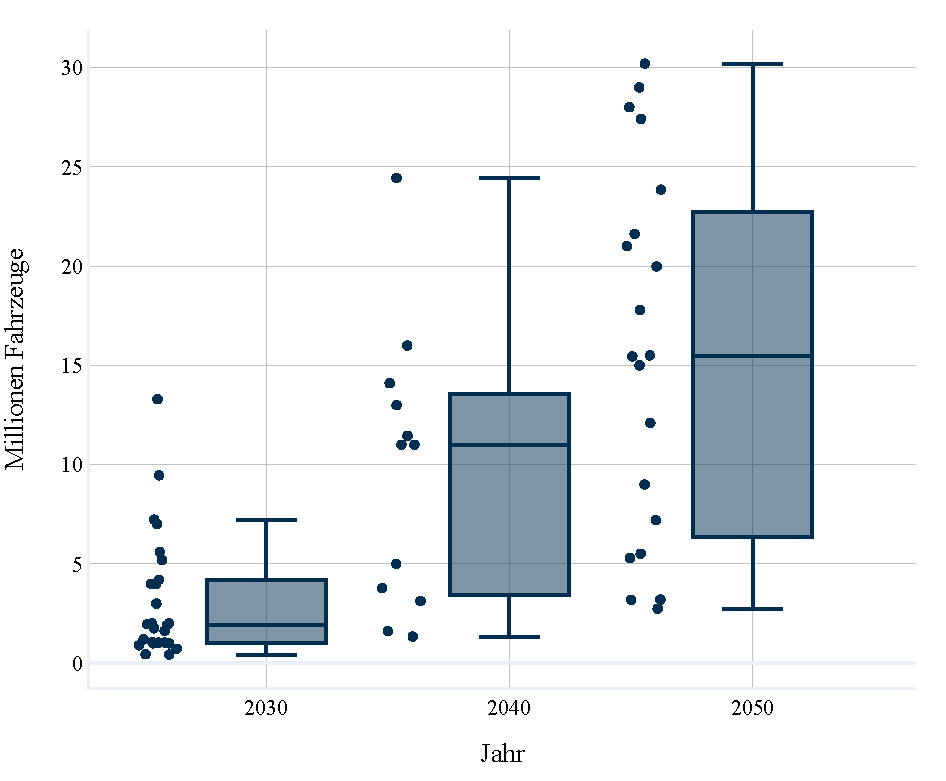
\includegraphics[width=\textwidth]{Bilder/RampUp-BEV-MA}
    \caption{Szenarienvergleich des Fahrzeugbestands von BEV bis zum Jahr \num{2050}}\label{fig:RampUpBEV}
\end{figure}

In \autoref{fig:RampUpBEV} sind die Annahmen der betrachteten Studien zum Fahrzeugbestand von \glspl{BEV} bis zum Jahr \num{2050} als Box-Plot dargestellt.
Die zugrundeliegenden Daten finden sich im Anhang in \autoref{tab:RampUpBEV}.
Trotz einer starken Streuung zeigt sich bis \num{2050} eine klare Zunahme im Bestand.
Der Median liegt 2030 noch bei \SI{1.9}{\MioStk}, steigt bis \num{2040} auf \SI{11.0}{\MioStk} und erreicht \num{2050} \SI{15.5}{\MioStk}.
Die starke Streuung lässt sich zum einen durch den unterschiedlichen Fokus der verschiedenen Studien und zum anderen durch den langen Zeithorizont und die damit verbundene Unsicherheit erklären.
In einzelnen Szenarien werden hohe Elektrifzierungsquoten angenommen und das Einhalten des \SIrange[range-phrase=~{--}~]{80}{95}{\percent}-Ziels des Klimaschutzplans \num{2050} vorausgesetzt, während andere Szenarien eine Fortschreibung der aktuellen Entwicklungen (\gls{BAU}) untersuchen.
So handelt es sich beispielsweise bei dem oberen Ausreißer im Jahr 2030 um das Elektrifizierungsszenario der dena-Leitstudie \glqq Integrierte Energiewende\grqq \cite{DEAGH2018}.
Hierbei handelt es sich um ein Szenario, welches sowohl hohe Elektrifizierungsquoten annimmt und als Leitlinie die Einhaltung des  \SIrange[range-phrase=~{--}~]{80}{95}{\percent}-Ziels setzt.\medskip

Neben dem Hochlauf an \glspl{BEV}, ist auch mit einem starken Hochlauf bei den \glspl{PHEV} zu rechnen.
Da ein Großteil der Fahrten von \glspl{PKW} eine Strecke von \SI{50}{\km} nicht überschreiten, können viele dieser Fahrten auch von \glspl{PHEV} batterieelektrisch zurückgelegt werden. \cite{Agora2019}
%Unterschiede gibt es jedoch in der maximalen Ladeleistung der Fahrzeugklassen.
%So werden \glspl{BEV} \num{2050} maximale Ladeleistungen von bis zu \SI{350}{\kw} aufweisen, während die maximale Ladeleistung von \glspl{PHEV} mit bis zu \SI{120}{\kw} deutlich geringer ausfällt. \cite{Kaul2019}

\begin{figure}[H]
    \centering
    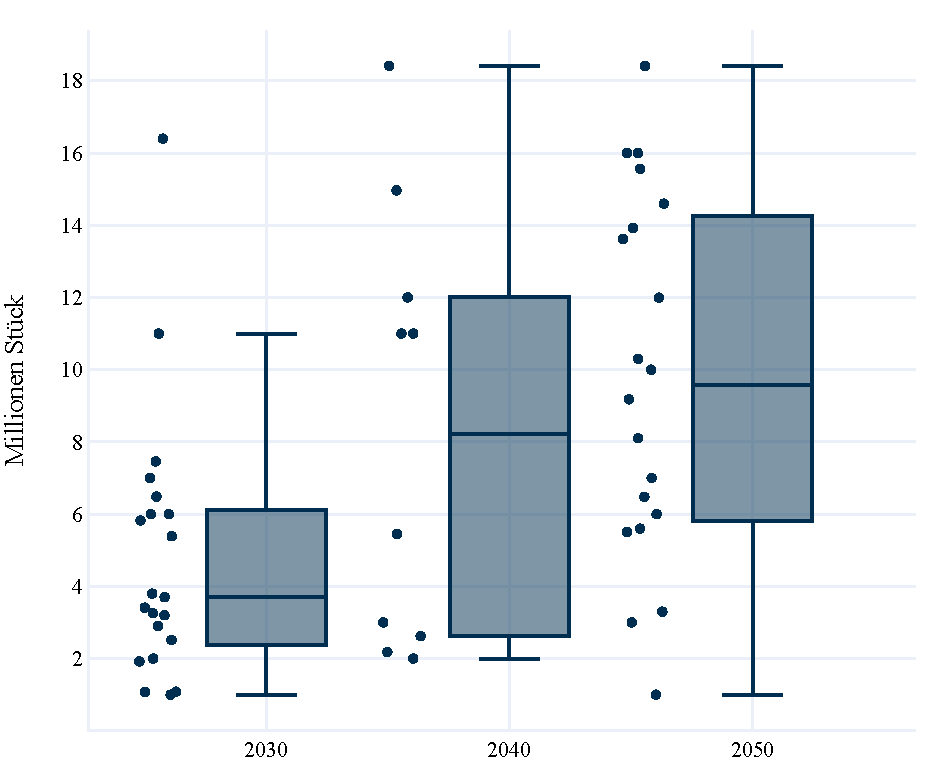
\includegraphics[width=\textwidth]{Bilder/RampUp-PHEV-MA}
    \caption{Szenarienvergleich des Fahrzeugbestands von PHEV bis zum Jahr \num{2050}}\label{fig:RampUpPHEV}
\end{figure}

\autoref{fig:RampUpPHEV} zeigt die Annahmen der betrachteten Studien zum Fahrzeugbestand von \glspl{PHEV} bis zum Jahr \num{2050} als Box-Plot.
Die zugrundeliegenden Daten finden sich im Anhang in \autoref{tab:RampUpPHEV}.
Bei \glspl{PHEV} liegt der Anstieg im Fahrzeugbestand anfangs sogar höher als bei \glspl{BEV}.
So liegt der Median 2030 bereits bei \SI{3.7}{\MioStk}.
Anschließend fällt der Fahrzeugbestand von \glspl{PHEV} hinter den der \glspl{BEV} zurück.
Bis \num{2040} steigt dieser auf \SI{8.2}{\MioStk} und \num{2050} auf \SI{9.6}{\MioStk}.
Je nach Studie und Szenario sinkt der Fahrzeugbestand nach \num{2040} sogar wieder, da zur Erreichung der Klimaziele oder aus ökonomischen Gründen der Umstieg auf \glspl{BEV} sinnvoller ist.

\begin{figure}[H]
    \centering
    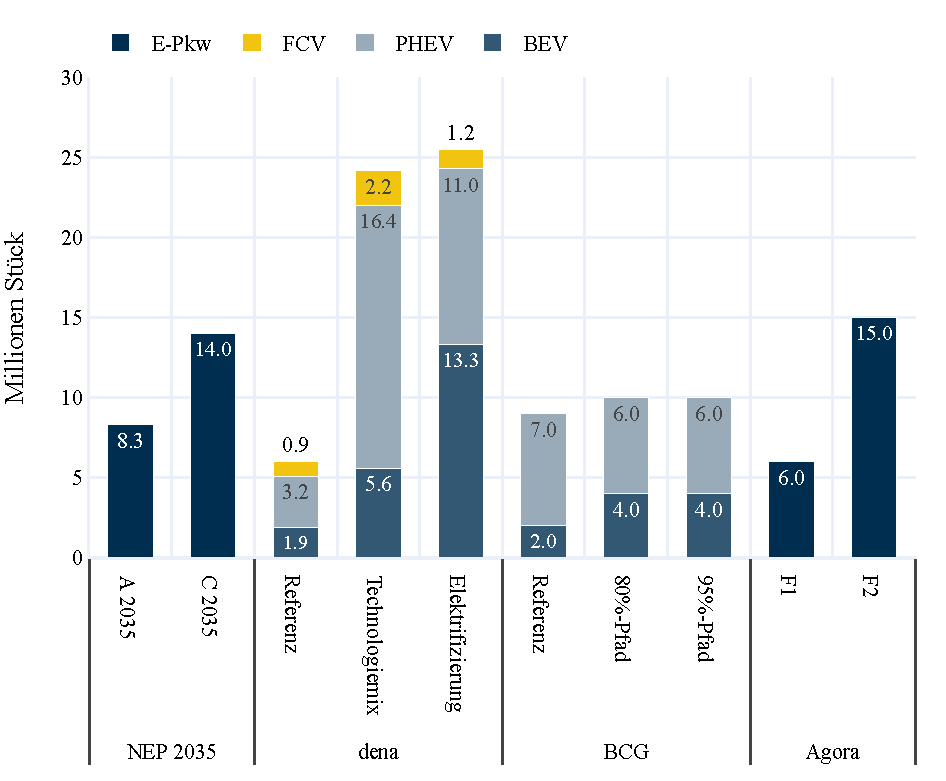
\includegraphics[width=\textwidth]{Bilder/RampUp-2030-Focus-MA}
    \caption{Fahrzeughochlauf alternativer Antriebstechnologien je Studie und Szenario bis zum Jahr \num{2030}}\label{fig:RampUp2030}
\end{figure}

Von den betrachteten Studien quantifizieren drei Studien den Netzausbaubedarf auf Verteilnetzebene und bilden somit eine Referenz zu der vorliegenden Arbeit und werden vertieft betrachtet.
Hierzu zählen die dena-Leitstudie \glqq Integrierte Energiewende\grqq{} \cite{DEAGH2018}, die BCG Studie \glqq Klimapfade für Deutschland\grqq{} \cite{BCG2018} und die Agora Studie \glqq Verteilnetzausbau für die Energiewende\grqq{} \cite{Agora2019}.
\autoref{fig:RampUp2030} zeigt den Fahrzeughochlauf verschiedener alternativer Antriebstechnologien im Verkehrssektor bis \num{2030} je Studie und Szenario.
Als Referenz wurden die konservativste und progressivste Annahmen des Netzentwicklungsplans \numrange[range-phrase=~{--}~]{2021}{2035} \cite{BNetzA2020} hinzugefügt.
Zu beachten ist hierbei, dass sich der Netzentwicklungsplan im Gegensatz zu den anderen Studien auf das Stützjahr \num{2035} bezieht.
Es wird erneut deutlich, dass sich der Markthochlauf je nach Studie und Szenario teils erheblich unterscheidet.
Grund hierfür sind nicht nur unterschiedliche Zielsetzungen der Studien, sondern auch verschiedene Modellgrundlagen und Annahmen.
So spannen sowohl die dena-Leitstudie als auch die BCG Studie einen Szenariorahmen für die Erreichung der Klimaschutzziele bis \num{2050} auf.
Dennoch liegt der Fahrzeugbestand alternativer Antriebstechnologien in den Klimaschutzszenarien \glqq Technologiemix\grqq{} und \glqq Elektrifizierung\grqq{} der dena-Leitstudie im Jahr 2030 mehr als doppelt so hoch als in den vergleichbaren Szenarien \glqq \SI{80}{\percent}-Pfad\grqq{} und \glqq \SI{95}{\percent}-Pfad\grqq{} der BCG Studie.
Beide Studien betrachten die Erreichung der Klimaschutzziele über alle relevanten Sektoren.
Hierbei bewertet die BCG Studie den Verkehrssektor als deutlich unelastischer als die dena-Leitstudie, wodurch im Jahr \num{2030} eine große Diskrepanz zwischen den Szenarien entsteht.\medskip

Demgegenüber definiert die Agora Studie feste Markthochläufe und ermittelt auf Grundlage dieser den nötigen Netzausbaubedarf in Abhängigkeit verschiedener Ladestrategien und -leistungen.
Die angenommenen Markthochläufe basieren in den \texttt{F}-Szenarien auf einer Fortschreibung des aktuellen Verkehrsverhaltens bei einer Antriebswende und in dem \texttt{M}-Szenario (s. \autoref{fig:RampUp2050}) auf einer Mobilitätswende.

\begin{figure}[H]
    \centering
    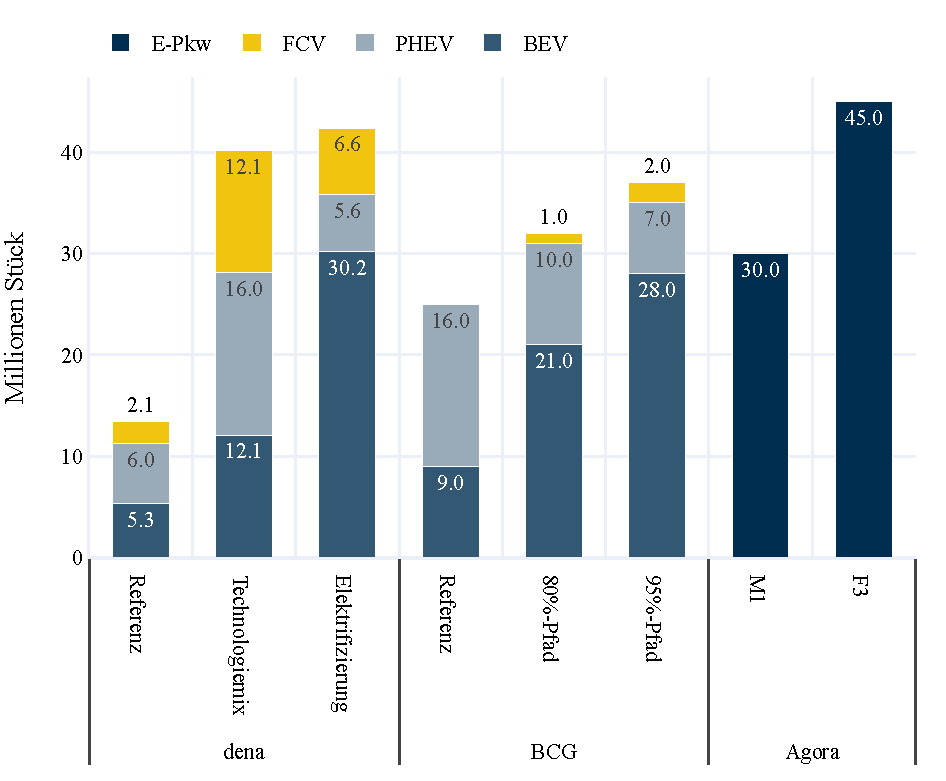
\includegraphics[width=\textwidth]{Bilder/RampUp-2050-Focus-MA}
    \caption{Fahrzeughochlauf alternativer Antriebstechnologien je Studie und Szenario bis zum Jahr \num{2050}}\label{fig:RampUp2050}
\end{figure}

In \autoref{fig:RampUp2050} findet sich der Fahrzeughochlauf verschiedener alternativer Antriebstechnologien im Verkehrssektor bis \num{2050} je Studie und Szenario.
Im Gegensatz zum Markthochlauf bis \num{2030}, liegen die Markthochlaufzahlen bis \num{2050} in allen Studien auf einem ähnlichen Niveau.
Dennoch liegen die Zahlen der BCG-Szenarien unter denen der dena-Leitstudie.
Der Grund hierfür ist, dass die Erreichung der Klimaschutzziele in der BCG Studie stärker in die Sektoren Energie, Haushalte, \gls{GHD} und Industrie verlagert wurden.
Beide Studien sind sich jedoch einig, dass zum Erreichen der Klimaschutzziele der Markthochlauf von alternativer Antriebstechnologien im Verkehrssektor gegenüber dem jeweiligen Referenzszenario (\gls{BAU}) deutlich angehoben werden muss.

\subsubsection{Kosten für den Netzausbau}

Die Kosten für den Netzausbau auf Verteilnetzebene werden von drei Studien untersucht.
Hierzu zählen die dena-Leitstudie \glqq Integrierte Energiewende\grqq{} \cite{DEAGH2018}, die BCG Studie \glqq Klimapfade für Deutschland\grqq{} \cite{BCG2018} und die Agora Studie \glqq Verteilnetzausbau für die Energiewende\grqq{} \cite{Agora2019}.

\begin{figure}[H]
    \centering
    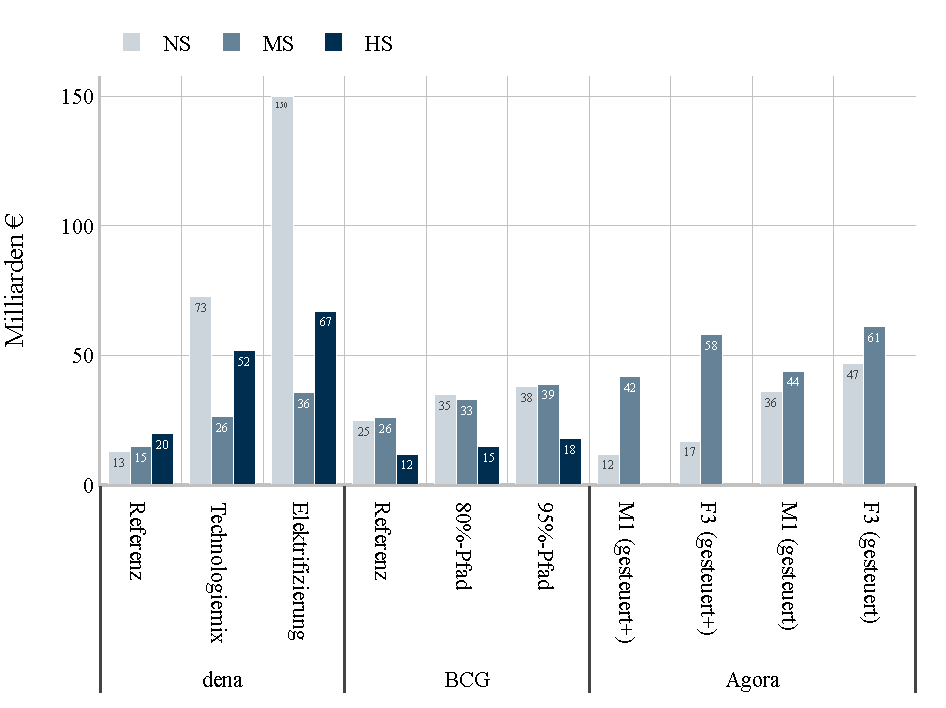
\includegraphics[width=\textwidth]{Bilder/DS-CAPEX-MA}
    \caption{Investitionsbedarf in die Verteilnetze bis zum Jahr \num{2050} je Spannungsebene}\label{fig:DSCAPEXMeta}
\end{figure}

In \autoref{fig:DSCAPEXMeta} finden sich die Ergebnisse der Studien für den Investitionsbedarf in die Verteilnetze bis zum Jahr \num{2050} aufgeteilt auf die drei Spannungsebenen \gls{NS}, \gls{MS} und \gls{HS}.
Deutlich wird hierbei, dass die dena-Leistudie die mit Abstand höchsten Kosten für den Netzausbau auf \gls{NS}- und \gls{HS}-Ebene ermittelt.
Die Agora Studie untersucht hingegen die Netzausbaukosten nicht auf der \gls{HS}-Ebene, ermittelt jedoch die höchsten Ausbaukosten auf \gls{MS}-Ebene.
Ein direkter Vergleich der Ergebnisse ist jedoch nur bedingt möglich, da die drei Studien unterschiedliche Grundsätze für ihre Szenarien und die Bestimmung des Netzausbaubedarfs ansetzen.
Deshalb sollen diese Grundsätze kurz näher betrachtet werden.

\paragraph{dena-Leitstudie \glqq Integrierte Energiewende\grqq:}

Ziel der dena-Leitstudie war es, Szenarien für eine Transformation des Energiesystems zur Einhaltung der Klimaschutzziele zu entwerfen.
Voraussetzung hierbei ist eine Minderung der Treibhausgasemissionen von \SIrange[range-phrase=~{--}~]{80}{95}{\percent} bis zum Jahr \num{2050}.
Dabei wurden die Sektoren Energiewirtschaft, Gebäude, Industrie, Verkehr, Land- und
Abfallwirtschaft inkludiert.
Somit handelt es sich bei den Netzausbaukosten um die Kosten der Summe der Effekte der Umstellung aller Sektoren auf einen Klimaschutzpfad.\medskip

Neben einem Referenzszenario, welches eine progressive Fortschreibung aktueller politischer und technologischer Entwicklungen darstellt, wird zwischen Technologiemix- und Elektrifizierungsszenarien unterschieden.
Während in den Elektrifizierungsszenarien von einer hohen Elektrifizierung der Sektoren Gebäude, Industrie und Verkehr ausgegangen wird, kommt es in den Technologiemixszenarien zu einem variableren Einsatz verschiedener Technologien und Energieträger.\medskip

Die Grundlage für die Bestimmung der Netzausbaukosten bildet die Ermittlung der zukünftigen Versorgungsaufgaben in den einzelnen Netzgebieten.
Die Versorgungsaufgabe wird hierbei im wesentlichen durch den Zubau \glspl{DEA} (\glspl{PVA}, \glspl{WEA} und \glspl{BMA}), sowie neuer Lasten (\glspl{EV} und \glspl{WP}), beeinflusst.
Die Zubauprognosen erfolgen zunächst auf Bundeslandebene und werden anschließend auf Gemeindeebene verteilt.
Weiterhin erfolgt eine Clusterung der Gemeinden in \glspl{NGK} anhand ihrer Einwohnerzahl, dem erwarteten Zubau an \glspl{DEA} und neuen Verbrauchern.
Hierdurch lassen sich die Berechnungen für einer Gemeinde auf eine andere Gemeinde innerhalb ihres Clusters übertragen.\medskip

Für die \gls{NS}- und \gls{MS}-Ebene erfolgt die Ermittlung des Netzausbaubedarfs mit Hilfe repräsentativer Netzstrukturen, welche genutzt werden um die nötigen Netzausbaumaßnahmen zu identifizieren.
Auf \gls{HS}-Ebene wird davon ausgegangen, dass der Netzausbaubedarf einen linearen Zusammenhang zum Zubau von \glspl{DEA} aufweist.
Abschließend wird der ermittelte Netzausbaubedarf auf allen Spannungsebenen monetär bewertet.\medskip

Eine Steuerung der Ladevorgänge von neuen Verbrauchern findet nicht statt.
Stattdessen geht die Studie davon aus, dass die zusätzliche Last durch \glspl{EV} und \glspl{WP} gleichzeitig mit der bisherigen Spitzenlast auftritt und der auslegungsrelevante Starklastfall somit deutlich erhöht wird.

\paragraph{BCG Studie \glqq Klimapfade für Deutschland\grqq:}

Auch die BCG Studie setzt sich das Erreichen der Klimaschutzziele bis \num{2050} als Ziel.
Dabei steht die volkswirtschaftliche Kosteneffizienz und die Wettbewerbsfähigkeit des Industriestandorts Deutschland im Vordergrund.
Weiterhin werden die gleichen Sektoren, wie in der dena-Leitstudie betrachtet. \medskip

Im Gegensatz zur dena-Leitstudie erfolgt für die Quantifizierung des Netzausbaubedarfs auf Grundlage eines vereinfachten Ansatzes.
Der Netzausbaubedarf wird in Anlehnung an die dena-Verteilnetzstudie \cite{DEAGH2012} auf Grundlage der Zubauzahlen für \glspl{DEA} und neue Verbraucher abgeschätzt und die Kosten anschließend anhand spezifischer Investitionskosten berechnet.

{
\renewcommand{\arraystretch}{1.2}% grßerer Zeilenabstand
\sisetup{range-phrase=~{--}~}% Gedankenstrich statt "bis" bei SIrange
\begin{table}[H]
	\begin{center}
		\caption{Studienvergleich der zentralen Annahmen zur Entwicklung des Zubaus an regenerativen Erzeugungseinheiten und neuen Verbraucher bis zum Jahr \num{2050}}
		\begin{tabu} to \textwidth {X[1.5] X[1, r] X[1, r]}
			\hline
            {}                                      &   dena-Leitstudie             & BCG Studie                \\
            {}                                      &   Elektrifizierungsszenarien  & \SI{95}{\percent}-Pfad    \\\hline
            Leistung PVA in \si{\gw}                &   \num{165}                   & \num{130}                 \\
            Leistung onshore WEA in \si{\gw}        &   \num{179}                   & \num{102}                 \\
            BEV in \si{\MioStk}                     &   \num{30.2}                  & \num{28}                  \\
            PHEV in \si{\MioStk}                    &   \num{5.6}                   & \num{7}                   \\
            Wärmepumpen in \si{\MioStk}             &   \num{17}                    & \num{16}                  \\\hline
		\end{tabu}
		\label{tab:denaVSBCG}
	\end{center}
	\vspace{-3mm}%Put here to reduce too much white space after your table
\end{table}
}

\autoref{tab:denaVSBCG} zeigt die wichtigsten Annahmen der dena-Leitstudie und der BCG Studie zur Entwicklung des Zubaus an \glspl{DEA} und neuen Verbraucher bis zum Jahr \num{2050} für die jeweils progressivsten Szenarien.
Die dena-Leitstudie ermittelt bis \num{2050} eine installierten Leistung von \SI{344}{\gw} an \glspl{PVA} und onshore \glspl{WEA}.
Dies ist etwa  \num{1.5}-mal so viel wie bei der BCG Studie.
Die ermittelten Zubauzahlen für die neuen Verbraucher sind hingegen bei beiden Studien ähnlich.\medskip

Dennoch ist der ermittelte Investitionsbedarf in die Verteilnetze in der dena-Leitstudie im Vergleich zur BCG Studie mehr als \num{2.5}-mal und auf \gls{NS}-Ebene sogar bis zu knapp \num{4}-mal so hoch.
Im Gegensatz zur dena-Leitstudie, wird in der BCG-Studie von einem gesteuerten Laden der neuen Verbraucher ausgegangen.
Dabei wird bei \glspl{WP} ein zweistündiger Warmwasserspeicher unterstellt, wodurch ein ebenso langer Starklastfall überbrückt werden kann.
\SI{80}{\percent} der \glspl{EV} reagieren auf Strommarktsignale und werden nur geladen, wenn der \gls{SOC} auf weniger als \SI{50}{\percent} fällt oder eine lange Fahrt ansteht.
Die starken Unterschiede im ermittelten Netzausbaubedarf sind somit sowohl eine folge der unterschiedlichen Berechnungsmethoden, der starken Differenzen im Verhalten der neuen Verbraucher als auch des unterschiedlichen starken Ausbaus an \glspl{DEA}.
Die Effekte können jedoch nicht klar differenziert werden.

\paragraph{Agora Studie \glqq Verteilnetzausbau für die Energiewende\grqq:}

Die Agora Studie setzt ihren Fokus ausschließlich auf die Elektromobilität und den hiermit verbundenen Netzausbaubedarf im Verteilnetz auf \gls{NS}- und \gls{MS}-Ebene.
Während die Annahmen zum Zubau von \glspl{DEA} und Wärmepumpen in den Szenarien konstant gehalten werden, wird in der Entwicklung der Elektromobilität zwischen Antriebs- und Mobilitätswende-Szenarien unterschieden.
Nicht elektrische Antriebstechnologien werden hierbei nicht berücksichtigt.
Zusätzlich wird ein starker Fokus auf den Einfluss von unterschiedlichen Ladestrategien auf den Netzausbaubedarf gelegt.\medskip

Die Ermittlung des Netzausbaudedarfs erfolgt analog zur Methodik der dena-Leitstudie.
Dabei wurden jedoch die Annahmen zur Gleichzeitigkeit der Ladevorgänge um eine Abhängigkeit von der Ladeleistung erweitert.
Zusätzlich wurde ein netzdienliches Ladekonzept (gesteuert) untersucht, welches eine Verschiebung der Ladevorgänge zur Residuallastglättung innerhalb der Standzeit ermöglicht, sowie ein erweitertes netzdienliches Ladekonzept (gesteuert\Plus), welches zusätzlich die Verschiebung der Ladevorgänge über mehrere Standzeiten und eine Kappung von Lastspitzen erlaubt.\medskip

Es zeigt sich, dass die Netzausbaukosten auf \gls{NS}-Ebene durch das erweiterte netzdienliche Ladekonzept deutlich gesenkt werden können, während der Einfluss auf \gls{MS}-Ebene nur gering ausfällt.
Auch zeigt sich aufgrund der Residuallastglättung des netzdienlichen Ladens im Vergleich zur dena-Leitstudie ein deutlich geringerer Netzausbaubedarf auf \gls{NS}-Ebene trotz der höheren Hochlaufzahlen an \glspl{EV} im \texttt{F3}-Szenario von \SI{45}{\MioStk} und einem vergleichbaren Ausbau an \glspl{DEA} von \SI{311}{\gw}.
Jedoch fällt der Netzausbaubedarf auf \gls{MS}-Ebene höher aus als in der dena-Leitstudie, da der Anteil an nicht steuerbaren Lasten (z.~B. Schnellladeinfrastruktur und Ladeinfrastruktur für Flotten und Busse) auf \gls{MS}-Ebene höher ausfällt und der hohe \gls{EV}-Bestand somit einen größeren Einfluss ausübt.

\subsection{Ergebnisse des Workshops \glqq Neue Verbraucher und elektrische Flexbilitäten\grqq{}}

In diesem Kapitel werden die wichtigsten Ergebnisse des Workshops \glqq Neue Verbraucher und elektrische Flexbilitäten\grqq{} aufgelistet.
Zu den Teilnehmern des Workshops zählten mehrheitlich Mitarbeiter von Netzbetreibern, Forschungsinstituten und energiewirtschaftlichen Unternehmen.
Die folgende Auflistung entspricht den relevanten Ergebnissen mehrerer Diskussionen und Umfragen innerhalb des Workshops.

\begin{itemize}
	\item Die Untersuchung eines Mobilitätswende-Szenarios ist von besonders hohem Interesse
	\item Private Ladeinfrastruktur zu Hause oder am Arbeitsplatz besitzt die größte Attraktivität für Verbraucher
%	\item Es wird davon ausgegangen, dass \num{2050} etwa \num{15} \glspl{EPKW} auf einen öffentlichen Ladepunkt kommen
	\item Eine regionale Konzentration von \glspl{EPKW} wird nur während der Markthochlaufphase eine relevante Rolle spielen
	\item Marktorientierte Ladestrategien können Gleichzeitigkeiten und damit den Netzausbaubedarf erhöhen
	\item Die Umsetzung von \gls{V2G}-Anwendungen wird als unwahrscheinlich eingestuft
	
\end{itemize}

\subsection{Szenarien}

\subsubsection{Ausbau regenerativer Energien}

Die Annahmen zu dem Hochlauf der regenerativen Erzeugerkapazitäten werden über die Szenarien hinweg als konstant angenommen.
Hierdurch werden Vermischungseffekte verhindert und der Einfluss der Elektromobilität kann getrennt bewertet werden.
Die Annahmen werden aus dem Szenario \ego des \openego Projektabschlussberichts \cite{Mueller2019} entnommen.

{
\renewcommand{\arraystretch}{1.2}% grßerer Zeilenabstand
\sisetup{range-phrase=~{--}~}% Gedankenstrich statt "bis" bei SIrange
\begin{table}[H]
	\begin{center}
		\caption{Hochlaufzahlen der regenerativen Erzeugerkapazitäten für die Stützjahre \num{2035} und \num{2050}}
		\begin{tabu} to \textwidth {X[1] X[1, r] X[1, r]}
			\hline
			Erzeugerkapazitäten   in \si{\gw} & \num{2035}  & \num{2050} \\ \hline
			Wind Onshore                      & \num{90.9}  & \num{98.4} \\
			Wind Offshore                     & \num{34.0}  & \num{27.0} \\
			Photovoltaik                      & \num{120.1} & \num{97.8} \\
			Biomasse                          & \num{8.7}   & \num{27.8} \\
			Wasserkraft                       & \num{5.6}   & \num{3.2}  \\ \hline
		\end{tabu}
		\label{tab:EE-RampUp}
	\end{center}
	\vspace{-3mm}%Put here to reduce too much white space after your table
\end{table}
}

{\color{red} TODO: Regionalisierung erklären}

\subsubsection{Wärmepumpen}

Der Hochlauf an Wärmepumpen in Deutschland wird ebenfalls über die Szenarien hinweg als konstant angenommen.
Die Hochlaufzahlen und der Jahresverbrauch entsprechen dem Szenario C~\num{2035} des Netzentwicklungsplans \numrange[range-phrase=~{--}~]{2021}{2035} \cite{BNetzA2020}.

{
\renewcommand{\arraystretch}{1.2}% grßerer Zeilenabstand
\sisetup{range-phrase=~{--}~}% Gedankenstrich statt "bis" bei SIrange
\begin{table}[H]
	\begin{center}
		\caption{Hochlaufzahlen für Wärmepumpen für die Stützjahre \num{2035} und \num{2050}}
		\begin{tabu} to \textwidth {X[1] X[1, r] X[1, r]}
			\hline
			Wärmepumpen                  & \num{2035} & \num{2050} \\ \hline
			Anzahl in \si{\MioStkSC}     & \num{7.0}  & \num{15.6} \\
			Leistung in \si{\gw}         & \num{21.0} & \num{46.8} \\
			Jahresverbrauch in \si{\twh} & \num{22.4} & \num{49.9} \\ \hline
		\end{tabu}
		\label{tab:WP-RampUp}
	\end{center}
	\vspace{-3mm}%Put here to reduce too much white space after your table
\end{table}
}

{\color{red} TODO: Regionalisierung erklären}

\subsubsection{Elektromobilität}\label{chap:EMob_Szenarien}

Bei der Elektromobilität müssen neben Annahmen zu den Zahlen zum Fahrzeughochlauf auch die technischen Daten der Fahrzeuge und die Verfügbarkeit der Ladeinfrastruktur berücksichtigt werden.

\paragraph{Fahrzeughochlauf:}
Der Fahrzeughochlauf unterscheidet sich je nach Szenario.
Insgesamt spiegeln alle Szenarien unterschiedlich starke Durchdringungen des \gls{MIV} mit \gls{EPKW} wider.\medskip

Das erste Szenario entspricht mit einem Fahrzeughochlauf von \SI{14}{\MioStk} den Annahmen des Szenarios C~\num{2035} des Netzentwicklungsplans \numrange[range-phrase=~{--}~]{2021}{2035} \cite{BNetzA2020}.
Die Hochlaufzahlen für das Referenzszenario entsprechen mit \SI{25.1}{\MioStk} den summierten Medianen der Literaturrecherche für den Fahrzeughochlauf an \glspl{BEV} und \glspl{PHEV} im Jahr \num{2050}.
Beim Mobilitätswende-Szenario wurde der Fahrzeugbestand des Effizienz-Plus Szenarios des Renewbility~III Projekts \cite{Institut2016} übernommen und von einer vollständigen Elektrifizierung ausgegangen.
Das Antriebswende-Szenario spiegelt hingegen den Fahrzeugbestand von \SI{47.7}{\MioStk} vom \DTMdate{2020-01-01} \cite{KBA2020} wieder.

{
\renewcommand{\arraystretch}{1.2}% grßerer Zeilenabstand
\sisetup{range-phrase=~{--}~}% Gedankenstrich statt "bis" bei SIrange
\begin{table}[H]
	\begin{center}
		\caption{Hochlaufzahlen je Szenario für E-Pkw}
		\begin{tabu} to 0.7\textwidth {X[1] X[1, r]}
			\hline
			Szenario         & E-PKW in \si{\MioStk}	\\ \hline
			NEP C~\num{2035} & \num{14.0}               \\
			Referenz         & \num{25.1}               \\
			Mobilitätswende  & \num{37.7}               \\
			Antriebswende    & \num{47.7}               \\ \hline
		\end{tabu}
		\label{tab:SzenarienRampUp}
	\end{center}
	\vspace{-3mm}%Put here to reduce too much white space after your table
\end{table}
}

Die Aufteilung in \glspl{BEV} und \glspl{PHEV} Szenarien anhand des ermittelten Medians der Literaturrecherche für den Fahrzeughochlauf an \glspl{BEV} und \glspl{PHEV} für das Stützjahr \num{2050}.
Innerhalb der Fahrzeugtypen erfolgt weiterhin eine Einteilung in die Fahrzeugklassen Kleinwagen, Mittelklasse und Oberklasse.
Es wird davon ausgegangen, dass sich die Einteilung zwischen \glspl{BEV} und \glspl{PHEV} nicht unterscheidet.
Die Einteilung in \autoref{tab:CarSplit} entspricht der Statistik des Kraftfahrt-Bundesamtes \cite{KBASegments2020} vom \DTMdate{2020-01-01}.
Es wird somit von einer Fortschreibung des aktuellen Verbraucherverhaltens ausgegangen.
Eine genaue Zuordnung der \gls{PKW}-Segmente in die Klassen findet sich im Anhang (\autoref{tab:KBASegments} und \autoref{tab:Segments}).

{
\renewcommand{\arraystretch}{1.2}% grßerer Zeilenabstand
\sisetup{range-phrase=~{--}~}% Gedankenstrich statt "bis" bei SIrange
\begin{table}[H]
	\begin{center}
		\caption{Aufteilung der Fahrzeuge auf die einzelnen Fahrzeugklassen}
		\begin{tabu} to 0.7\textwidth {X[1] X[1, r]}
			\hline
			Fahrzeugklassen   & Anteil in \si{\percent}  \\ \hline
			BEV Kleinwagen    & \num{15.9}               \\
			BEV Mittelklasse  & \num{35.3}               \\
			BEV Oberklasse    & \num{10.5}               \\
			PHEV Kleinwagen   & \num{9.8}                \\
			PHEV Mittelklasse & \num{21.9}               \\
			PHEV Oberklasse   & \num{6.5}                \\ \hline
		\end{tabu}
		\label{tab:CarSplit}
	\end{center}
	\vspace{-3mm}%Put here to reduce too much white space after your table
\end{table}
}

\paragraph{Technische Daten:}

Die technischen Daten der Fahrzeuge sind klassenspezifisch und innerhalb ihrer Klasse homogen.
In \autoref{tab:TechPowerCap} finden sich die fahrzeugseitige maximale Ladeleistung und die nutzbare Batteriekapazität der jeweiligen Fahrzeugklassen.
Eine Limitierung der Ladeleistung durch die Unterscheidung in Normal- und Schnellladung, erfolgt im Simulationsmodell von Seiten der Ladeinfrastruktur.

{
\renewcommand{\arraystretch}{1.2}% grßerer Zeilenabstand
\sisetup{range-phrase=~{--}~}% Gedankenstrich statt "bis" bei SIrange
\begin{table}[H]
	\begin{center}
		\caption{Maximale Ladeleistung und nutzbare Batteriekapazität je Fahrzeugklasse}
		\begin{tabu} to \textwidth {X[0.9] X[1.3, r] X[1.5, r]}
				\hline
				Fahrzeugklasse    & Maximale Ladeleistung in \si{\kw} & Nutzbare Batteriekapazität in \si{\kwh} \\ \hline
				BEV Kleinwagen    & \num{120}                         & \num{70}                                \\
				BEV Mittelklasse  & \num{350}                         & \num{100}                               \\
				BEV Oberklasse    & \num{350}                         & \num{120}                               \\
				PHEV Kleinwagen   & \num{120}                         & \num{25}                                \\
				PHEV Mittelklasse & \num{120}                         & \num{30}                                \\
				PHEV Oberklasse   & \num{120}                         & \num{40}                                \\ \hline
            \multicolumn{3}{l}{Quelle: Szenario \glqq Verstärkte Elektrifizierung\grqq{} für das Jahr \num{2049} \cite{Kaul2019}}
		\end{tabu}
		\label{tab:TechPowerCap}
	\end{center}
	\vspace{-3mm}%Put here to reduce too much white space after your table
\end{table}
}

Der elektrische Energieverbrauch der Fahrzeuge wird aus den Annahmen der Studie \glqq eMobil \num{2050}\grqq{} \cite{Hacker2014} abgeleitet.
Es wird angenommen, dass Kleinwagen gegenüber Mittelklasse Fahrzeugen einen um \SI{20}{\percent} reduzierten Energieverbrauch aufweisen.
Oberklasse Fahrzeuge weisen hingegen einen um \SI{20}{\percent} erhöhten Energieverbrauch auf.\medskip

Weiterhin bietet die Studie \glqq eMobil \num{2050}\grqq{} nur Verbrauchsangaben nach dem \glspl{NEFZ}, welche nicht realen Verbrauchsdaten entsprechen.
Nach \cite{Heinfellner2015} lag der Realverbrauch \num{2013} gegenüber einer Messung nach \gls{NEFZ} im Mittel um \SI{27}{\percent} höher.
Die Werte für das Jahr \num{2050} der Studie \glqq eMobil \num{2050}\grqq{} wurden um diesen Faktor erhöht.

{
\renewcommand{\arraystretch}{1.2}% grßerer Zeilenabstand
\sisetup{range-phrase=~{--}~}% Gedankenstrich statt "bis" bei SIrange
\begin{table}[H]
	\begin{center}
		\caption{Durchschnittlicher elektrischer Energieverbrauch je Fahrzeugklasse}
		\begin{tabu} to 0.7\textwidth {X[1] X[1, r]}
			\hline
			Fahrzeugklasse    & Verbrauch in \si{\kwhkm} \\ \hline
			BEV Kleinwagen    & \num{11.9}              \\
			BEV Mittelklasse  & \num{14.8}              \\
			BEV Oberklasse    & \num{17.8}              \\
			PHEV Kleinwagen   & \num{12.1}              \\
			PHEV Mittelklasse & \num{15.2}              \\
			PHEV Oberklasse   & \num{18.2}              \\ \hline
		\end{tabu}
		\label{tab:TechVerbrauch}
	\end{center}
	\vspace{-3mm}%Put here to reduce too much white space after your table
\end{table}
}

\paragraph{Ladeinfrastruktur:}

Die Ladeinfrastruktur wird im Gegensatz zu den Annahmen zum Fahrzeughochlauf nicht in absoluten Zahlen ausgedrückt.
Stattdessen werden den einzelnen Wegezwecken der Fahrzeuge Wahrscheinlichkeiten zugeordnet, dass ein Fahrzeug am Zielort geladen werden kann.
Weiterhin wird diese Wahrscheinlichkeit auf verschiedene Ladeleistungen aufgeteilt.
Dabei wird grundsätzlich zwischen Normal- und Schnellladung unterschieden.
Normalladung beschreibt in dieser Masterarbeit alle Ladevorgänge mit einer Leistung von bis zu einschließlich \SI{50}{\kw} und Schnellladung alle Ladevorgänge von größer \SIrange[range-phrase=~bis~einschließlich~]{50}{350}{\kw}.

\subparagraph{Normalladung} beinhaltet in dieser Arbeit die Leistungsklassen \SI{3.7}{\kw}, \SI{11}{\kw}, \SI{22}{\kw} und \SI{50}{\kw}.
Eine Zuordnung der Leistungsklassen auf die einzelnen Wegezwecke erfordert vorerst eine Zuordnung der \UCs auf die Wegezwecke.
In \autoref{tab:WegLadeUseCase} findet sich die entsprechende prozentuale Aufteilung der \UCs auf die Wegezwecke.

{
\renewcommand{\arraystretch}{1.2}% grßerer Zeilenabstand
\sisetup{range-phrase=~{--}~}% Gedankenstrich statt "bis" bei SIrange
\begin{table}[H]
	\begin{center}
		\caption{Prozentuale Zuordnung der \UCs auf die verschiedenen Wegezwecke}
		\begin{tabu} to \textwidth {X[1.2] X[1.1, r] X[1.3, r] X[1.7, r] X[1.8, r] X[1.2, r]}
            \hline
            Wegezweck  & Eigenheim           & Wohnanlage          & Firmenparkplatz     & Gewerbeparkplatz   & Straßenrand         \\ \hline
            Arbeit     & \SI{0.0}{\percent}  & \SI{0.0}{\percent}  & \SI{64.5}{\percent} & \SI{0.0}{\percent}  & \SI{35.5}{\percent} \\
            dienstlich & \SI{0.0}{\percent}  & \SI{0.0}{\percent}  & \SI{38.0}{\percent} & \SI{6.0}{\percent}  & \SI{56.0}{\percent} \\
            Ausbildung & \SI{0.0}{\percent}  & \SI{0.0}{\percent}  & \SI{64.5}{\percent} & \SI{0.0}{\percent}  & \SI{35.5}{\percent} \\
            Einkauf    & \SI{0.0}{\percent}  & \SI{0.0}{\percent}  & \SI{0.0}{\percent}  & \SI{76.5}{\percent} & \SI{23.5}{\percent} \\
            Erledigung & \SI{0.0}{\percent}  & \SI{0.0}{\percent}  & \SI{0.0}{\percent}  & \SI{38.0}{\percent} & \SI{62.0}{\percent} \\
            Freizeit   & \SI{0.0}{\percent}  & \SI{0.0}{\percent}  & \SI{0.0}{\percent}  & \SI{38.5}{\percent} & \SI{61.5}{\percent} \\
            nach Hause & \SI{43.4}{\percent} & \SI{25.1}{\percent} & \SI{0.0}{\percent}  & \SI{0.0}{\percent}  & \SI{31.4}{\percent} \\ \hline
		\end{tabu}
		\label{tab:WegLadeUseCase}
	\end{center}
	\vspace{-3mm}%Put here to reduce too much white space after your table
\end{table}
}

Derzeit leben in Deutschland ungefähr \SI{44.2}{\MioMen} in Gebäuden mit maximal zwei Wohnungen und \SI{37.2}{\MioMen} in Mehrfamilienhäusern.
Etwa \SI{80}{\percent} der Fahrzeugbesitzer in Gebäuden mit maximal zwei Wohnungen verfügen über einen Stellplatz in der Garage oder unter einem \texttt{Carport}.
In Mehrfamilienhäusern verfügen hingegen nur \SI{55}{\percent} der Fahrzeugbesitzer über einen Stellplatz für ihr Fahrzeug. \cite{dena2020}
Unter der vereinfachenden Annahme einer gleichmäßigen Verteilung von Fahrzeugen zwischen Bewohnern von Ein- und Mehrfamilienhäusern ergibt sich hieraus die ermittelte Aufteilung der \UCs auf den Wegezweck \nHdot.\medskip

Die Aufteilung der \UCs auf die Wegezwecke \Einkaufdot, \Erledigung und \Freizeitdot, ergeben sich aus den Wegeanteilen nach Fahrtzweck im \gls{MIV}-Privatverkehr. \cite{Rikus2015}
Im Falle des Wegezwecks \Einkaufdot, wird angenommen, dass Lebensmittelgschäfte einen Gewerbeparkplatz für jeden Kunden vorhalten.
Weiterhin wird angenommen, dass im Falle von sonstigen Waren und sonstigen Dienstleistungen in \SI{50}{\percent} der Fälle ein Gewerbeparkplatz zur Verfügung steht.
Bei dem Wegezweck \Erledigungdot, wird davon ausgegangen, dass beim Besuch von Behörden, Banken, Post und Geldautomaten ein Gewerbeparkplatz vorhanden ist und bei sonstigen Erledigungen in \SI{50}{\percent} der Fälle.
Für den Wegezweck \Freizeitdot, wird angenommen, dass bei kulturelle Einrichtungen und Veranstaltungen ein Gewerbeparkplatz vorhanden ist.
Bei sonstigen Freizeitaktivitäten wird angenommen, dass in \SI{50}{\percent} der Fälle ein Gewerbeparkplatz vorhanden ist.
In allen verbleibenden Fällen erfolgt ein Parken am Straßenrand.\medskip

Für die Abschätzung der Wahrscheinlichkeit auf einem Firmenparkplatz für den Wegezweck \Arbeit parken zu können, wurde die Parkplatzsituation am Arbeitsplatz zugrunde gelegt.
Demnach werden \SI{67}{\percent} aller Arbeitswege mit dem \gls{PKW} zurückgelegt, wenn die Parkplatzsituation am Arbeitsplatz als nicht schwierig eingestuft wird.
Demgegenüber werden bei einer schwierigen Parkplatzsituation nur \SI{36}{\percent} der Arbeitswege mit dem \gls{PKW} zurückgelegt.
Insgesamt werden mit dem \gls{PKW} \SI{56}{\percent} aller Arbeitswege zurückgelegt. \cite{Ecke2020}
Unter der Annahme, dass eine nicht schwierige Parkplatzsituation am Arbeitsplatz gleichbedeutend mit einem Firmenparkplatz und eine schwierige Parkplatzsituation mit dem Parken am Straßenrand ist, ergeben sich hieraus die ermittelten Anteile für den Wegezweck \Arbeitdot.
Weiterhin wird angenommen, dass dieses Verhältnis auf den Wegezweck \Ausbildung~übertragen werden kann.\medskip

Für den Wegezweck \dienstdot, wird die Aufteilung nach dem üblichen Stellplatz am Fahrtziel im Wirtschaftsverkehr verwendet. \cite{Rikus2015}
Demnach parken gewerbliche Halter im Wirtschaftsverkehr in \SI{30}{\percent} der Fälle am Straßenrand.
In \SI{26}{\percent} der Fälle erfolgt das Parken auf einem Privatgrundstück.
Im Wirtschaftsverkehr handelt es sich in der Regel nicht um das eigene Privatgrundstück, weswegen diese Art des Parkens ebenfalls als Parken am Straßenrand gewertet wird.
In \SI{6}{\percent} der Fälle erfolgt das Parken auf einem Gewerbeparkplatz und in \SI{38}{\percent} der Fälle auf einem Firmenparkplatz.\medskip

Anschließend erfolgt je \UC eine Abschätzung der Wahrscheinlichkeiten, ob eine Ladung stattfinden kann und mit welcher Ladeleistung geladen werden kann.
In \autoref{tab:UCProbability2050} finden sich die entsprechenden Annahmen.

%{
%\renewcommand{\arraystretch}{1.2}% grßerer Zeilenabstand
%\sisetup{range-phrase=~{--}~}% Gedankenstrich statt "bis" bei SIrange
%\begin{table}[H]
%	\begin{center}
%		\caption{Wahrscheinlichkeitverteilung der Ladeleistungen je \UC für das Stützjahr \num{2035}}
%		\begin{tabu} to \textwidth {X[1.7] X[1.3, r] X[1, r] X[1, r] X[1, r] X[1, r]}
%			\hline
%			\UC  & keine Ladung        & \SI{3.7}{\kw}       & \SI{11}{\kw}        & \SI{22}{\kw}        & \SI{50}{\kw}        \\ \hline
%			Eigenheim        & \SI{15.0}{\percent} & \SI{17.0}{\percent} & \SI{59.5}{\percent} & \SI{8.5}{\percent}  & \SI{0.0}{\percent}  \\
%			Wohnanlage       & \SI{75.0}{\percent} & \SI{3.8}{\percent}  & \SI{20.0}{\percent} & \SI{1.3}{\percent}  & \SI{0.0}{\percent}  \\
%			Firmenparkplatz  & \SI{50.0}{\percent} & \SI{5.0}{\percent}  & \SI{20.0}{\percent} & \SI{20.0}{\percent} & \SI{5.0}{\percent}  \\
%			Gewerbeparkplatz & \SI{50.0}{\percent} & \SI{0.0}{\percent}  & \SI{5.0}{\percent}  & \SI{30.0}{\percent} & \SI{15.0}{\percent} \\
%			Straßenrand      & \SI{75.0}{\percent} & \SI{2.5}{\percent}  & \SI{10.0}{\percent} & \SI{10.0}{\percent} & \SI{2.5}{\percent}  \\ \hline
%		\end{tabu}
%		\label{tab:UCProbability2035}
%	\end{center}
%	\vspace{-3mm}%Put here to reduce too much white space after your table
%\end{table}
%}
%
{
\renewcommand{\arraystretch}{1.2}% grßerer Zeilenabstand
\sisetup{range-phrase=~{--}~}% Gedankenstrich statt "bis" bei SIrange
\begin{table}[H]
	\begin{center}
		\caption{Wahrscheinlichkeitverteilung der Ladeleistungen je \UC}
		\begin{tabu} to \textwidth {X[1.7] X[1.3, r] X[1, r] X[1, r] X[1, r] X[1, r]}
			\hline
			Lade Use   Case  & keine Ladung        & \SI{3.7}{\kw}      & \SI{11}{\kw}        & \SI{22}{\kw}        & \SI{50}{\kw}        \\ \hline
			Eigenheim        & \SI{15.0}{\percent} & \SI{0.0}{\percent} & \SI{63.8}{\percent} & \SI{21.3}{\percent} & \SI{0.0}{\percent}  \\
			Wohnanlage       & \SI{50.0}{\percent} & \SI{5.0}{\percent} & \SI{40.0}{\percent} & \SI{5.0}{\percent}  & \SI{0.0}{\percent}  \\
			Firmenparkplatz  & \SI{50.0}{\percent} & \SI{0.0}{\percent} & \SI{20.0}{\percent} & \SI{20.0}{\percent} & \SI{10.0}{\percent} \\
			Gewerbeparkplatz & \SI{25.0}{\percent} & \SI{0.0}{\percent} & \SI{7.5}{\percent}  & \SI{45.0}{\percent} & \SI{22.5}{\percent} \\
			Straßenrand      & \SI{50.0}{\percent} & \SI{0.0}{\percent} & \SI{20.0}{\percent} & \SI{20.0}{\percent} & \SI{10.0}{\percent} \\ \hline
		\end{tabu}
		\label{tab:UCProbability2050}
	\end{center}
	\vspace{-3mm}%Put here to reduce too much white space after your table
\end{table}
}

In allen \UCs wird davon ausgegangen, dass die Ladevorgänge in Zukunft mit immer höheren Ladeleistungen stattfinden.
Für den \UC \Eigenheim wird angenommen, dass jeder Besitzer eines \gls{EPKW} eine Ladevorrichtung vorhält, wenn die technischen Voraussetzungen gegeben sind.
Bei rund \SI{15}{\percent} der Stellplätze von Gebäuden mit einer oder zwei Wohnungen besteht kein Zugang zum Stromnetz. \cite{dena2020}
Es wird angenommen, dass von diesem Bestand die Hälfte einen Zugang zum Stromnetz erhält.
Die Aufteilung der Ladeleistungen erfolgt hierbei in Anlehnung an \cite{NPZMAVE2020}.
Es wird davon ausgegangen. dass der Anteil von Ladevorgängen mit einer Leistung von \SI{3.7}{\kw} keine Rolle mehr spielt.
Der Anteil an Ladevorgängen mit \SI{11}{\kw} wird weiter wachsen, allerdings langsamer als der Anteil an Ladevorgängen mit \SI{22}{\kw}.
Eine Ladung mit \SI{50}{\kw} wird im privaten Bereich ebenfalls keine Rolle spielen.
Das prozentuale Verhältnis zwischen den Ladeleistungen beträgt \(0:75:25:0\)\medskip

Stellplätze von Mehrfamilienhäusern besitzen mit ungefähr \SI{50}{\percent} der Fälle deutlich seltener Zugang zum Stromnetz. \cite{dena2020}
Es wird angenommen, dass alle Stellplätze mit den entsprechenden technischen Vorraussetzungen mit einer Ladevorrichtung ausgestattet werden und bei der Hälfte der Stellplätze ohne Zugang zum Stromnetz dieser nachgerüstet wird.
In Wohnanlagen werden hohe Ladeleistungen eine Ausnahme bleiben.
Insgesamt wird von einem Verhältnis zwischen den Ladeleistungen von \(10:80:10:0\) ausgegangen.\medskip

Bei Firmen- bzw. Gewerbeparkplätzen wird davon ausgegangen, dass zukünftig Mitarbeiter bzw. Kunden in \SI{75}{\percent} der Fälle Zugriff auf einen Ladepunkt haben.
Die Verteilung der Ladeleistungen geschieht in Anlehnung an das Ladesäulenregister der Bundesnetzagentur \cite[][Stand: \DTMdate{2020-09-09}]{BundesnetzagenturElektrizitaet2020} und der Stromtankstellen Statistik des \texttt{GoingElectric} Forums \cite[][Stand: \DTMdate{2020-10-21}]{Weemaes2020}.
Demnach besitzt ein Großteil (\SIrange[range-phrase=~bzw.~]{80}{51}{\percent}) der heutigen öffentlich zugänglichen Ladepunkte eine Ladeleistung von \SIrange{22}{42}{\kw}.
Insgesamt wird davon ausgegangen, dass sich der Trend zu hohen Ladeleistungen weiter fortsetzt.
Dies gilt jedoch vor allem für Gewerbeparkplätze, da hohe Ladeleistungen und die Verfügbarkeit von Ladepunkten zur Kundenakquise genutzt werden.
Bei Firmenparkplätzen wird mit einem Verhältnis von \(0:40:40:20\) gerechnet.
Demgegenüber wird bei Gewerbeparkplätzen mit einem Verhältnis von \(0:10:60:30\) gerechnet.\medskip

Im Falle des \UCs \Straszenranddot, wird angenommen, dass zukünftig noch in \SI{75}{\percent} der Fälle kein Ladepunkt zur Verfügung steht.
Weiterhin entspricht das Verhältnis der Ladeleistungen dem von Firmenparkplätze.\medskip

Aus den zuvor getroffenen Annahmen können nun die Wahrscheinlichkeiten für die Ladevorgänge je Wegezweck berechnet werden.
Die entsprechenden Ergebnisse finden sich in \autoref{tab:WegezweckProbability2050}.

%{
%\renewcommand{\arraystretch}{1.2}% grßerer Zeilenabstand
%\sisetup{range-phrase=~{--}~}% Gedankenstrich statt "bis" bei SIrange
%\begin{table}[H]
%	\begin{center}
%		\caption{Wahrscheinlichkeitverteilung der Ladeleistungen je Wegezweck für das Stützjahr \num{2035}}
%		\begin{tabu} to \textwidth {X[1.2] X[1.2, r] X[1, r] X[1, r] X[1, r] X[1, r]}
%			\hline
%			Wegezweck  & keine Ladung        & \SI{3.7}{\kw}      & \SI{11}{\kw}        & \SI{22}{\kw}        & \SI{50}{\kw}        \\ \hline
%			Arbeit     & \SI{58.9}{\percent} & \SI{4.1}{\percent} & \SI{16.5}{\percent} & \SI{16.5}{\percent} & \SI{4.1}{\percent}  \\
%			dienstlich & \SI{64.0}{\percent} & \SI{3.3}{\percent} & \SI{13.5}{\percent} & \SI{15.0}{\percent} & \SI{4.2}{\percent}  \\
%			Ausbildung & \SI{58.9}{\percent} & \SI{4.1}{\percent} & \SI{16.5}{\percent} & \SI{16.5}{\percent} & \SI{4.1}{\percent}  \\
%			Einkauf    & \SI{55.9}{\percent} & \SI{0.6}{\percent} & \SI{6.2}{\percent}  & \SI{25.3}{\percent} & \SI{12.1}{\percent} \\
%			Erledigung & \SI{65.5}{\percent} & \SI{1.6}{\percent} & \SI{8.1}{\percent}  & \SI{17.6}{\percent} & \SI{7.3}{\percent}  \\
%			Freizeit   & \SI{65.4}{\percent} & \SI{1.5}{\percent} & \SI{8.1}{\percent}  & \SI{17.7}{\percent} & \SI{7.3}{\percent}  \\
%			nach Hause & \SI{48.9}{\percent} & \SI{9.1}{\percent} & \SI{34.0}{\percent} & \SI{7.1}{\percent}  & \SI{0.8}{\percent}  \\ \hline
%		\end{tabu}
%		\label{tab:WegezweckProbability2035}
%	\end{center}
%	\vspace{-3mm}%Put here to reduce too much white space after your table
%\end{table}
%}
%
{
\renewcommand{\arraystretch}{1.2}% grßerer Zeilenabstand
\sisetup{range-phrase=~{--}~}% Gedankenstrich statt "bis" bei SIrange
\begin{table}[H]
	\begin{center}
		\caption{Wahrscheinlichkeitverteilung der Ladeleistungen je Wegezweck}
		\begin{tabu} to \textwidth {X[1.2] X[1.2, r] X[1, r] X[1, r] X[1, r] X[1, r]}
			\hline
			Wegezweck  & keine Ladung        & \SI{3.7}{\kw}      & \SI{11}{\kw}        & \SI{22}{\kw}        & \SI{50}{\kw}        \\ \hline
			Arbeit     & \SI{50.0}{\percent} & \SI{0.0}{\percent} & \SI{20.0}{\percent} & \SI{20.0}{\percent} & \SI{10.0}{\percent} \\
			dienstlich & \SI{48.5}{\percent} & \SI{0.0}{\percent} & \SI{19.3}{\percent} & \SI{21.5}{\percent} & \SI{10.8}{\percent} \\
			Ausbildung & \SI{50.0}{\percent} & \SI{0.0}{\percent} & \SI{20.0}{\percent} & \SI{20.0}{\percent} & \SI{10.0}{\percent} \\
			Einkauf    & \SI{30.9}{\percent} & \SI{0.0}{\percent} & \SI{10.4}{\percent} & \SI{39.1}{\percent} & \SI{19.6}{\percent} \\
			Erledigung & \SI{40.5}{\percent} & \SI{0.0}{\percent} & \SI{15.3}{\percent} & \SI{29.5}{\percent} & \SI{14.8}{\percent} \\
			Freizeit   & \SI{40.4}{\percent} & \SI{0.0}{\percent} & \SI{15.2}{\percent} & \SI{29.6}{\percent} & \SI{14.8}{\percent} \\
			nach Hause & \SI{34.8}{\percent} & \SI{1.3}{\percent} & \SI{44.0}{\percent} & \SI{16.8}{\percent} & \SI{3.1}{\percent}  \\ \hline
		\end{tabu}
		\label{tab:WegezweckProbability2050}
	\end{center}
	\vspace{-3mm}%Put here to reduce too much white space after your table
\end{table}
}

\subparagraph{Schnellladung} entspricht in dieser Arbeit einer Art Notfallladung.
Fällt der \gls{SOC} eines Fahrzeugs während einer Fahrt unter \SI{20}{\percent}, wird eine Schnellladestation angefahren und das Fahrzeug für \SI{15}{\Minuten} geladen.
Bei Schnellladevorgängen wird in dieser Arbeit grundsätzlich zwischen einer Ladung mit \SI{150}{\kw} und mit \SI{350}{\kw} unterschieden.
Nach dem Ladesäulenregister der Bundesnetzagentur \cite[][Stand: \DTMdate{2020-09-09}]{BundesnetzagenturElektrizitaet2020} weisen bereits heute \SI{59}{\percent} der Ladeinfrastruktur mit einer Leistung von mehr als \SI{50}{\kw} eine Ladeleistung von über \SI{150}{\kw} auf.
Es ist davon auszugehen, dass sich auch bei der Schnellladeinfrastruktur der Trend zu hohen Ladeleistungen fortsetzt.
Weiterhin ist davon auszugehen, dass dies vor allem für Tankstellen außerhalb von Ortschaften gilt, da diese häufig an Autobahnen liegen.
Auf Autobahnen werden häufig lange Strecken zurückgelegt und der Ladebedarf durch Schnellladeinfrastruktur ist somit besonders hoch.
Innerhalb von Ortschaften ist eine kleinere Ladeleistung von \SI{150}{\kw} oftmals ausreichend.
In \autoref{tab:SchnellProbability2050} finden sich die getroffenen Annahmen für die Szenarien.

%{
%\renewcommand{\arraystretch}{1.2}% grßerer Zeilenabstand
%\sisetup{range-phrase=~{--}~}% Gedankenstrich statt "bis" bei SIrange
%\begin{table}[H]
%	\begin{center}
%		\caption{Wahrscheinlichkeitverteilung der Ladeleistungen von Schnellladeinfrastruktur für das Stützjahr \num{2035}}
%		\begin{tabu} to \textwidth {X[1] X[1, r] X[1, r]}
%			\hline
%			Lade Use   Case      & \SI{150}{\kw}       & \SI{350}{\kw}       \\ \hline
%			Tankstelle innerorts & \SI{80.0}{\percent} & \SI{20.0}{\percent} \\
%			Tankstelle außerorts & \SI{20.0}{\percent} & \SI{80.0}{\percent} \\ \hline
%		\end{tabu}
%		\label{tab:SchnellProbability2035}
%	\end{center}
%	\vspace{-3mm}%Put here to reduce too much white space after your table
%\end{table}
%}
%
{
\renewcommand{\arraystretch}{1.2}% grßerer Zeilenabstand
\sisetup{range-phrase=~{--}~}% Gedankenstrich statt "bis" bei SIrange
\begin{table}[H]
	\begin{center}
		\caption{Wahrscheinlichkeitverteilung der Ladeleistungen von Schnellladeinfrastruktur}
		\begin{tabu} to 0.7\textwidth {X[1] X[1, r] X[1, r]}
			\hline
			Lade Use   Case      & \SI{150}{\kw}       & \SI{350}{\kw}       \\ \hline
			Tankstelle innerorts & \SI{80.0}{\percent} & \SI{20.0}{\percent} \\
			Tankstelle außerorts & \SI{0.0}{\percent}  & \SI{100.0}{\percent} \\ \hline
		\end{tabu}
		\label{tab:SchnellProbability2050}
	\end{center}
	\vspace{-3mm}%Put here to reduce too much white space after your table
\end{table}
}

\subsection{Sensitivitäten}

Zusätzlich zu den zuvor beschriebenen Szenarien sollen in dieser Arbeit zwei Sensitivitäten in Form von Szenaretten untersucht werden.
Hierbei untersucht die \Kleinwagen den Einfluss einer weiter voranschreitenden Mobilitätswende und bei der \SzeFirmenparkplatz wird der Einfluss eines geringeren Anteils an Ladevorgängen am Arbeitsplatz untersucht.

\subsubsection{\Kleinwagendot}

Die \Kleinwagen basiert auf den Annahmen des Mobilitätswende-Szenarios.
Hierbei werden die netzseitigen Auswirkungen einer Verschiebung der Fahrzeugklassen hin zu mehr Kleinwagen untersucht.
Kleinwagen machen in dieser Szenarette \SI{50}{\percent}, Mittelklasse Fahrzeuge \SI{35}{\percent} und Oberklasse Fahrzeuge \SI{15}{\percent} des Gesamtbestandes aus.
Zusätzlich wird ein Anwachsen des Anteils von \glspl{BEV} auf \SI{75}{\percent} der Fahrzeuge angenommen.
Die hierdraus entstehende Aufteilung findet sich in \autoref{tab:CarSplitSzenarette}.

{
\renewcommand{\arraystretch}{1.2}% grßerer Zeilenabstand
\sisetup{range-phrase=~{--}~}% Gedankenstrich statt "bis" bei SIrange
\begin{table}[H]
	\begin{center}
		\caption{Anpassung der Aufteilung der Fahrzeuge auf die einzelnen Fahrzeugklassen für die Szenarette}
		\begin{tabu} to 0.7\textwidth {X[1] X[1, r]}
			\hline
			Fahrzeugklassen   & Anteil in \si{\percent} \\ \hline
			BEV Kleinwagen    & \num{37.5}              \\
			BEV Mittelklasse  & \num{26.3}              \\
			BEV Oberklasse    & \num{11.3}              \\
			PHEV Kleinwagen   & \num{12.5}              \\
			PHEV Mittelklasse & \num{8.8}               \\
			PHEV Oberklasse   & \num{3.8}               \\ \hline
		\end{tabu}
		\label{tab:CarSplitSzenarette}
	\end{center}
	\vspace{-3mm}%Put here to reduce too much white space after your table
\end{table}
}

\subsubsection{\SzeFirmenparkplatzdot}

Aufgrund der hohen Gleichzeitigkeit und der zeitlichen Überschneidung mit einer hohen Erzeugung aus \glspl{PVA} kommt dem Laden am Arbeitsplatz eine besondere Bedeutung zu.
Die \SzeFirmenparkplatz soll die Sensitivität des Antriebswende-Szenarios auf die Verfügbarkeit von Ladepunkten auf Firmenparkplätzen untersuchen.
Hierfür wird angenommen, dass nur noch in \SI{25}{\percent} der Fälle eine Ladung am Firmenparkplatz stattfinden kann.
Die Annahme wird somit gegenüber des Antriebswende-Szenarios halbiert.

{
\renewcommand{\arraystretch}{1.2}% grßerer Zeilenabstand
\sisetup{range-phrase=~{--}~}% Gedankenstrich statt "bis" bei SIrange
\begin{table}[H]
	\begin{center}
		\caption{Anpassung der Wahrscheinlichkeitverteilung der Ladeleistungen für die Szenarette}
		\begin{tabu} to \textwidth {X[1.7] X[1.3, r] X[1, r] X[1, r] X[1, r] X[1, r]}
			\hline
			Lade Use Case   & keine Ladung        & \SI{3.7}{\kw}      & \SI{11}{\kw}        & \SI{22}{\kw}        & \SI{50}{\kw}        \\ \hline
			Firmenparkplatz & \SI{50.0}{\percent} & \SI{0.0}{\percent} & \SI{20.0}{\percent} & \SI{20.0}{\percent} & \SI{10.0}{\percent} \\ \hline
		\end{tabu}
		\label{tab:UCProbabilitySzenarette}
	\end{center}
	\vspace{-3mm}%Put here to reduce too much white space after your table
\end{table}
}

In \autoref{tab:UCProbabilitySzenarette} findet sich die hier draus entstehende Wahrscheinlichkeitsverteilung für den \UC \Firmeparkplatzdot.
Dadurch kommt es für die Wegezwecke \Arbeitdot, \dienst und \Ausbildung zu einer veränderten Wahrscheinlichkeitsverteilung, welche in \autoref{tab:WegezweckProbabilitySzenarette} zu finden ist.

{
\renewcommand{\arraystretch}{1.2}% grßerer Zeilenabstand
\sisetup{range-phrase=~{--}~}% Gedankenstrich statt "bis" bei SIrange
\begin{table}[H]
	\begin{center}
		\caption{Anpassung der Wahrscheinlichkeitverteilung der Ladeleistungen je Wegezweck für die Szenarette}
		\begin{tabu} to \textwidth {X[1.2] X[1.2, r] X[1, r] X[1, r] X[1, r] X[1, r]}
			\hline
			Wegezweck  & keine Ladung        & \SI{3.7}{\kw}      & \SI{11}{\kw}        & \SI{22}{\kw}        & \SI{50}{\kw}       \\ \hline
			Arbeit     & \SI{58.9}{\percent} & \SI{0.0}{\percent} & \SI{16.5}{\percent} & \SI{16.5}{\percent} & \SI{8.2}{\percent} \\
			dienstlich & \SI{62.5}{\percent} & \SI{0.0}{\percent} & \SI{13.7}{\percent} & \SI{15.9}{\percent} & \SI{8.0}{\percent} \\
			Ausbildung & \SI{58.9}{\percent} & \SI{0.0}{\percent} & \SI{16.5}{\percent} & \SI{16.5}{\percent} & \SI{8.2}{\percent} \\ \hline
		\end{tabu}
		\label{tab:WegezweckProbabilitySzenarette}
	\end{center}
	\vspace{-3mm}%Put here to reduce too much white space after your table
\end{table}
}